\documentclass[a4paper, 11pt]{article}
\usepackage[utf8]{inputenc}
\usepackage[russian]{babel}
\usepackage{amssymb}
\usepackage{amsmath}
\usepackage{graphicx}
\usepackage{float}

\newcommand{\w}{\widetilde}

\voffset = -1cm 
\footskip=100pt
\hoffset = -1cm

\newcommand{\wide}{
\stackrel{0}{x}
}
\begin{document}
\begin{center}

\textsc{Численное моделирование нестационарного 
    одномерного течения газа с использованием схемы 
    для логарифма плотности с центральными разностями}

\end{center}

\enlargethispage{9\baselineskip}

\section{Постановка дифференциальной задачи}
Одномерное движение вязкого баротропного газа описывается системой дифференциальных уравнений:
$$
\begin{cases} 
\displaystyle{\frac{\partial \rho}{\partial t} +
 \frac{\partial \rho u}{\partial x} = f_0}, \\

\displaystyle{\rho \frac{\partial u}{\partial t} +
 \rho u \frac{\partial u}{\partial x}+ 
 \frac{\partial p}{\partial x} = 
\mu \frac{\partial^2 u}{\partial x^2}
+ \rho f}
\end{cases}
$$

\begin{center}
$
p = p (\rho)
$ - известная функция давления от плотности. 
$f_0 \equiv 0, $
$f$ - известная функция от $(t, x)$.
\end{center}
$$\mu \in [0,001; 0,1]$$

Неизвестные функции плотности и скорости:

\begin{center}
$\rho,\ u: [0, T] \times [0, X] \rightarrow \mathbb{R}$, где $T,\ X > 0$
\end{center}

$$\rho > 0$$

Краевые условия:
$$(\rho, u)|_{t=0} = (\rho_0, u_0), x \in [0, X]$$

Для гарантирования положительности $\rho$ вместо функции $\rho$ имеет смысл искать функцию $g = \ln(\rho)$ 

Тогда система дифференциальных уравнений примет вид

$$
\begin{cases}
\displaystyle{\frac{\partial g}{\partial t} + \frac{1}{2} \left(u\frac{\partial g}{\partial x} +     \frac{\partial ug}{\partial x} +(2-g)\frac{\partial u}{\partial x}\right) = f_0},\\
\displaystyle{\frac{\partial u}
{\partial t} + \frac{1}{3} \left(u 
\frac{\partial u}{\partial x} +
 \frac{\partial u^2}{\partial x}\right) +
  \tilde{p}'(g)
 \frac{\partial g}{\partial x} = \mu
  e^{-g}\frac{\partial^2 u}{\partial x^2} +
   f}
\end{cases}
$$

\section{Построение разностной схемы}
Для численного решения системы введем сетку на области $[0, T] \times [0, X]$ с шагом $h$ по оси $OX$ и $\tau$ по оси $OT$. Узел сетки с координатами $(n, m)$ соответствует точке $(n\tau, mh)$ области. Для разностных операторов и значений в узлах сетки будем использовать обозначения, введенные в пособии к вычислительному практикуму.

$M$ - количество узлов вдоль оси $OX$.
$N$ - количество узлов вдоль оси $OT$.

Запишем разностную схему:

$$
\begin{cases}
\displaystyle{G_t + \frac{1}{2}(V\hat{G}_{\wide} + (V\hat{G})_{\wide} + (2-G)V_{\wide}) = f_0},\ \ \ 1 \leqslant m \leqslant M - 1,\\
\displaystyle{G_{t,0} + \frac{1}{2} ((V\hat{G})_{x,0} + (2 - G_0)V_{x, 0})} - \\
\displaystyle{
-\frac{h}{2}((GV)_{x\overline{x}, 1} - 
\frac{1}{2}(GV)_{x\overline{x}, 2} + (2 - G_0)
(V_{x\overline{x}, 1} - 
\frac{1}{2}V_{x\overline{x}, 2})) = (f_0)_0},\\
\displaystyle{
G_{t, M} + \frac{1}{2}((V\hat{G})_{\overline{x}, M} + (2 - G_M)V_{\overline{x}, M}) +} \\ 
\displaystyle{+\frac{h}{2}((GV)_{x\overline{x}, M-1} - 
\frac{1}{2}(GV)_{x\overline{x}, M-2} + 
(2-G_M)(V_{x\overline{x}, M - 1} - 
\frac{1}{2}V_{x\overline{x}, M-2})) = (f_0)_M},\\
\displaystyle{V_t + \frac{1}{3}(V\hat{V}_{\wide} + (V\hat{V}_{\wide})) + \tilde{p}'(\hat{G})\hat{G}_{\wide} = \tilde{\mu}\hat{V}_{x\overline{x}} - 
(\tilde{\mu} - \mu e^{-\hat{G}})V_{x\overline{x}} + f},\ \ \  1 \leqslant m \leqslant M - 1,
\end{cases}
$$
где $\tilde{\mu} = \mu\vert\vert e^{-\hat{G}}\vert\vert_C$.
\\[5pt]
Запишем эту схему в следующем виде, сгруппировав слагаемые:

$$
\begin{cases}
\displaystyle{
G_{m-1}^{n+1} \left(\frac{-V_{m}^n}{2h}\right) + G_m^{n+1} \left(\frac{1}{\tau} + \frac{1}{2}\left(V_{\wide}\right)_m^n\right) +}\\
\displaystyle{ +
G_{m+1}^{n+1} \left(\frac{V_m^n}{2h}\right) + V_{m+1}^{n+1} \left(\frac{1}{2h}\right) + V_{m-1}^{n+1}\left(\frac{1}{2h}\right) =} \\
\displaystyle{
= 
f_0 (n\tau, mh) + G_m^n \left(\frac{1}{\tau} 
+\frac{1}{2} \left(V_{\wide}\right)_m^n\right)
,\ \ \  1 \leqslant m \leqslant M - 1} & (1)\\
\displaystyle{
G_0^{n+1} \left(\frac{1}{\tau} + \frac{(V_x)_0^n}{2}\right)
 + V^{n+1}_1 \left(\frac{1}{h}\right) = 
 f_0 (n\tau, 0) + \frac{G_0^n}{\tau} + } \\
 \displaystyle{ +\frac{h}{2} \left( ((GV)_{x\overline{x}})_1^n -\frac{1}{2}((GV)_{x\overline{x}})_1^n + (2 - G_0^n)((V_{x\overline{x}})_1^n - \frac{1}{2}(V_{x\overline{x}})_2^n)\right) + G_0^n \frac{(V_x)_0^n}{2} }, & (2)\\
 \displaystyle{
G_{M}^{n+1} \left(\frac{1}{\tau} + \frac{\left(V_{\overline{x}}\right)_M^n}{2}\right) + V_{M-1}^{n+1} \left(-\frac{1}{h}\right) = 
f_0(n\tau, X) + \frac{G_M^n}{\tau} + G_M^n \frac{V_{\overline{x}}}{2} - } \\
\displaystyle{
-\frac{h}{2}\left(((GV)_{x\overline{x}})_{M-1}^n
-\frac{1}{2}((GV)_{x\overline{x}})_{M-2}^n + (2-G_M^n)(V_{x\overline{x}})_{M-1}^n - 
\frac{1}{2}(V_{x\overline{x}})_{M-2}^n\right)}, & (3)\\
\displaystyle{
V_{m-1}^{n+1} \left(-\frac{V_m^n}{3h}-\left(\frac{\mu \vert\vert e^{-\hat{G}}\vert\vert_C}{h^2} \right) \right) + 
V_m^{n+1} \left(\frac{1}{\tau} + \frac{(V_{\wide})_m^n}{3} + \frac{2\mu \vert\vert e^{-\hat{G}}\vert\vert_C}{h^2}\right) +} \\
\displaystyle {
V_{m+1}^{n+1}\left(\frac{V_m^n}{3h} - 
\frac{\mu \vert\vert e^{-\hat{G}}\vert\vert_C}{h^2}\right) + G_{m-1}^{n+1}\left(-\tilde{p}'\frac{G_m^n}{2h}\right) + 
G_{m+1}^{n+1}\left(
\tilde{p}'\frac{G_m^n}{2h}\right) = } \\
\displaystyle{
 f(n\tau, mh) - (V_{x\overline{x}})_m^n \left(\mu \vert\vert e^{-\hat{G}}\vert\vert_C - \mu e^{-G_m^n} + \frac{V_m^n}{\tau}\right),\ \ \ 1 \leqslant m \leqslant M-1} & (4)
\end{cases}
$$
Будем называть \textit{$n$-ым слоем} узлы сетки с координатой по времени равной $n$.
\enlargethispage{9\baselineskip}
Заметим, что значения $V$ и $G$ известны на нулевом слое.
При известных значениях функции на слое $n$, с помощью системы уравнений, можно вычислить значения функций на $n+1$ слое. Покажем, как уравнения $(1)-(4)$ формируют необходимую СЛАУ $(*)$.

Уравнение $(1)$ для $m = 1$ и $m=M-1$ содержит четыре неизвестных, т.к. $V_0 = V_M = 0$ на любом слое. Для $2 \leqslant m \leqslant M - 2$ уравнение $(1)$ содержит пять неизвестных.\\ 
$m$, пробегая в уравнении $(1)$ значения от $1$ до $M - 1$, формирует $M-1$ уравнение в системе $(*)$ для неизвестных $G_0^{n+1}, \ldots , G_M^{n+1}$ и $V_1^{n+1}, \ldots , V_{M-1}^{n+1}$

Уравнение $(2)$ дает 1 уравнение в СЛАУ $(*)$ для неизвестных $G_0^{n+1}, V_1^{n+1}$.

Уравнение $(3)$ дает 1 уравнение в СЛАУ $(*)$ для неизвестных $G_M^{n+1}, V_{M-1}^{n+1}$.

Уравнение $(4)$ для $m =1$ и $m = M-1$ содержит четыре неизвестных, по тем же причинам, что и уравнение $(1)$, и пять при $2 \leqslant m \leqslant M - 2$.\\
$m$, пробегая в уравнении $(4)$ значения от $1$ до $M - 1$, формирует $M-1$ уравнение в системе $(*)$ для неизвестных $G_0^{n+1}, \ldots , G_M^{n+1}$ и $V_1^{n+1}, \ldots , V_{M-1}^{n+1}$

И так, СЛАУ $(*)$ является системой с $(M+1) + (M-1) = 2M$ неизвестными и $(M-1) + 1 + 1 + (M-1) = 2M$ уравнениями. В каждом уравнении не более пяти ненулевых коэффициентов.

Таким образом СЛАУ $(*)$ является разреженной, что делает естественным применение итерационных алгоритмов для ее решения.

Последовательно решая такие СЛАУ для $1 \leqslant n \leqslant N$, получим значения $G$ и $V$ во всех узлах сетки.

\section{Результаты тестовых расчетов для гладких решений}
Для проверки реализованного на ЭВМ алгоритма сделаем следующее.
\begin{enumerate}
\item Положим 
$$
\begin{cases}
\rho (t, x) = e^t (\cos (\pi x / 10) + 1.5), \\
u (t, x) = \cos (2 \pi t) \sin (\pi (x/10)^2), \\
\tilde{p}' = 1, \\
\mu =  0,001.
\end{cases}
$$
\item Аналитически вычислим $f_0$ и $f$ поставленной дифференциальной задачи с такими $\rho$ и $u$.
\item Сравним значения функций $g (t, x) = \ln (\rho (t, x))$ и $u$ в узлах сетки, вычисленные алгоритмом со значениями, вычисленными аналитически.
\end{enumerate}
Рассмотрим нормы невязок скорости и плотности на последнем слое и их динамику при изменении шага сетки.
\enlargethispage{5\baselineskip}\\

$||G_m^n - g (\tau n, hm)||_{C_h}$:
\begin{center}
\begin{tabular}{|c|c|c|c|c|}
\hline 
 N\textbackslash M &      20      &      40      &      80      &     160      \\ 
 \hline 
        20         & 3,362763e-03 & 6,011030e-03 & 7,096117e-03 & 7,236886e-03 \\ 
 \hline 
        80         & 1,880232e-03 & 5,676989e-04 & 1,246442e-03 & 1,386106e-03 \\ 
 \hline 
        320        & 2,802104e-03 & 4,896486e-04 & 1,661393e-04 & 2,851023e-04 \\ 
 \hline 
       1280        & 3,010187e-03 & 7,215251e-04 & 1,136553e-04 & 4,505472e-05 \\ 
 \hline 
\end{tabular}
\end{center}
$||G_m^n - g (\tau n, hm)||_{L2_h}$:
\begin{center}
\begin{tabular}{|c|c|c|c|c|}
\hline 
 N\textbackslash M &      20      &      40      &      80      &     160      \\ 
 \hline 
        20         & 5,557584e-03 & 6,537687e-03 & 6,800276e-03 & 6,779306e-03 \\ 
 \hline 
        80         & 1,778678e-03 & 8,423468e-04 & 1,323880e-03 & 1,430520e-03 \\ 
 \hline 
        320        & 2,713867e-03 & 4,234380e-04 & 2,703903e-04 & 3,703753e-04 \\ 
 \hline 
       1280        & 2,961370e-03 & 6,407478e-04 & 1,004257e-04 & 7,166092e-05 \\ 
 \hline 
\end{tabular}
\end{center}
$||G_m^n - g (\tau n, hm)||_{W_2^1}$:
\begin{center}
\begin{tabular}{|c|c|c|c|c|}
\hline 
 N\textbackslash M &      20      &      40      &      80      &     160      \\ 
 \hline 
        20         & 1,136667e-02 & 9,124210e-03 & 8,964636e-03 & 8,817623e-03 \\ 
 \hline 
        80         & 8,425275e-03 & 3,368378e-03 & 2,423212e-03 & 2,311330e-03 \\ 
 \hline 
        320        & 8,537628e-03 & 2,798925e-03 & 1,073595e-03 & 6,855815e-04 \\ 
 \hline 
       1280        & 8,610764e-03 & 2,792095e-03 & 9,235949e-04 & 3,470701e-04 \\ 
 \hline 
\end{tabular}
\end{center}
$||V_m^n - u (\tau n, hm)||_{C_h}$:
\begin{center}
\begin{tabular}{|c|c|c|c|c|}
\hline 
 N\textbackslash M &      20      &      40      &      80      &     160      \\ 
 \hline 
        20         & 4,468816e-03 & 4,268340e-03 & 4,351276e-03 & 4,389003e-03 \\ 
 \hline 
        80         & 2,622438e-03 & 1,336355e-03 & 1,699522e-03 & 1,839407e-03 \\ 
 \hline 
        320        & 3,676246e-03 & 5,604782e-04 & 3,710596e-04 & 4,832500e-04 \\ 
 \hline 
       1280        & 3,999036e-03 & 8,878083e-04 & 1,334016e-04 & 9,542056e-05 \\ 
 \hline 
\end{tabular}
\end{center}
$||V_m^n - u (\tau n, hm)||_{L2_h}$:
\begin{center}
\begin{tabular}{|c|c|c|c|c|}
\hline 
 N\textbackslash M &      20      &      40      &      80      &     160      \\ 
 \hline 
        20         & 7,078412e-03 & 7,015676e-03 & 7,350591e-03 & 7,451807e-03 \\ 
 \hline 
        80         & 3,496533e-03 & 2,095983e-03 & 2,655382e-03 & 2,826796e-03 \\ 
 \hline 
        320        & 4,455167e-03 & 7,794411e-04 & 5,839730e-04 & 7,395209e-04 \\ 
 \hline 
       1280        & 4,883520e-03 & 1,085492e-03 & 1,899382e-04 & 1,501232e-04 \\ 
 \hline 
\end{tabular}
\end{center}
$||V_m^n - u (\tau n, hm)||_{W_2^1}$:
\begin{center}
\begin{tabular}{|c|c|c|c|c|}
\hline 
 N\textbackslash M &      20      &      40      &      80      &     160      \\ 
 \hline 
        20         & 1,602271e-02 & 8,410281e-03 & 8,402222e-03 & 8,590046e-03 \\ 
 \hline 
        80         & 1,518330e-02 & 4,503082e-03 & 3,239430e-03 & 3,419199e-03 \\ 
 \hline 
        320        & 1,633145e-02 & 4,786022e-03 & 1,538671e-03 & 9,706054e-04 \\ 
 \hline 
       1280        & 1,673155e-02 & 5,113734e-03 & 1,570499e-03 & 5,209392e-04 \\ 
 \hline 
\end{tabular}
\end{center}

Динамикой падения невязок подтверждается сходимость решения порядка $\tau + h^2$
\enlargethispage{7\baselineskip}\\

\section{Результаты расчетов для негладких начальных данных}
Решим 2 задачи с негладкими начальными данными.
\begin{equation}
\begin{split}
& f_0 \equiv  0, \\
& f_1  \equiv 0, \\
& \tilde{p}' = 1
\end{split}
\end{equation}

$$
(1)\quad \quad
\begin{cases}
\rho_0(x) = 1, \quad x < 4,5 \text{ или } x > 5,5,\\
\rho_0(x) = 2, \quad x \in [4,5; 5,5],\\
u_0(x) \equiv 0, \quad x \in [0; 10],\\
u(t, 0) = u(t, 10) = 0, \quad t \in [0; 1], \\
& \mu =  0,001, \\
\end{cases}
$$

$$
(2)\quad \quad
\begin{cases}
u_0(x) = 0, \quad x < 4,5 \text{ или } x > 5,5,\\
u_0(x) = 1, \quad x \in [4,5; 5,5],\\
\rho_0(x) \equiv 1, \quad x \in [0; 10],\\
u(t, 0) = u(t, 10) = 0, \quad t \in [0; T],\\
& \mu =  0,1. \\
\end{cases}
$$
Настройки алгоритма:
$$
M = 600,
N = 600.
$$
Для задачи (1) получаем:
\newpage
\begin{figure}[h]
	\begin{minipage}[h] {0.49\linewidth}
		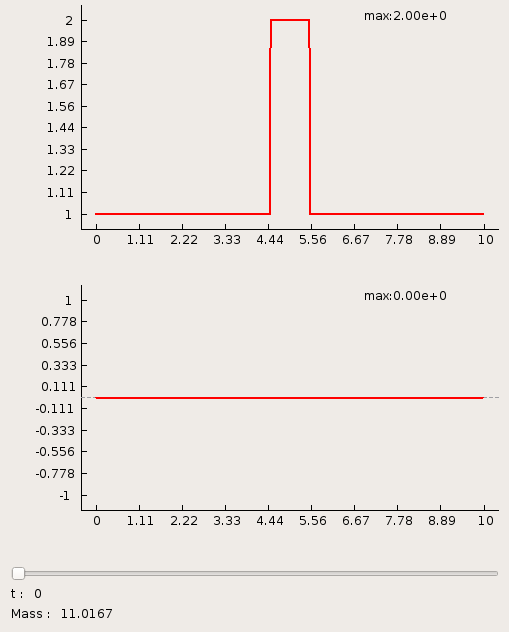
\includegraphics[width=1\linewidth]{p1/p1_t=0.png}
	\end{minipage}
	\begin{minipage}[h] {0.49\linewidth}
		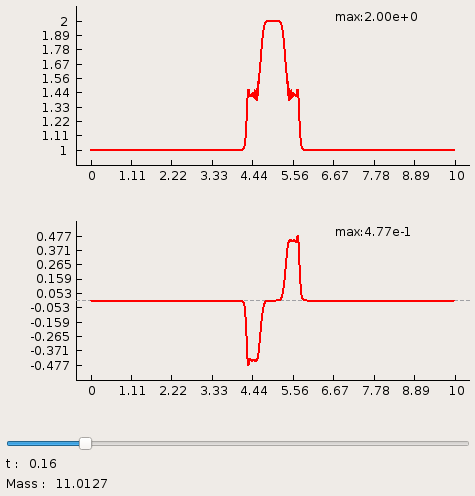
\includegraphics[width=1\linewidth]{p1/p1_t=0,16.png}
	\end{minipage}
	\begin{minipage}[h] {0.49\linewidth}
		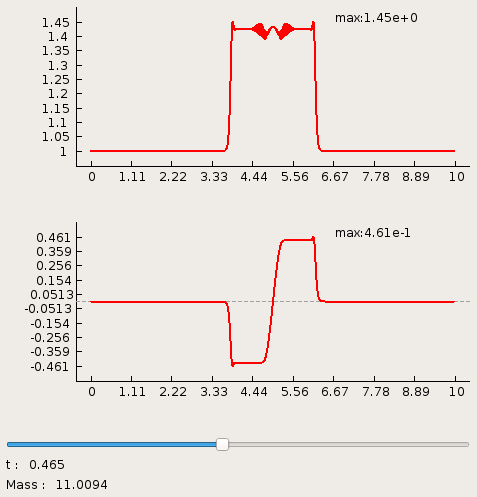
\includegraphics[width=1\linewidth]{p1/p1_t=0,465.png}
	\end{minipage}
		\begin{minipage}[h] {0.49\linewidth}
		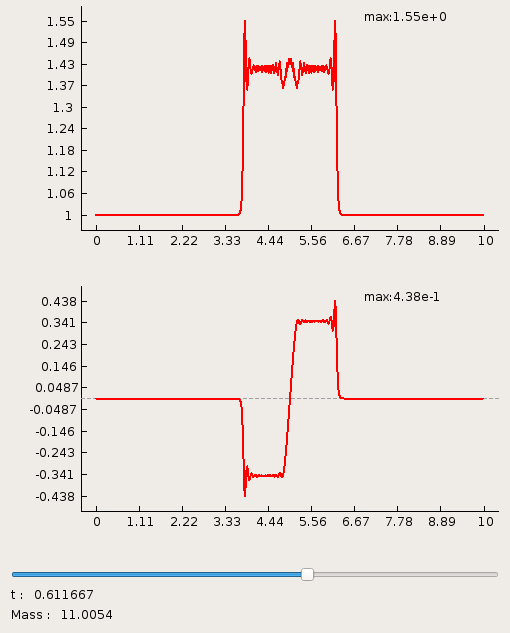
\includegraphics[width=1\linewidth]{p1/p1_t=0,611.png}
	\end{minipage}
	\end{figure}
	\newpage
\begin{figure}[h]
	\begin{minipage}[h] {0.49\linewidth}
		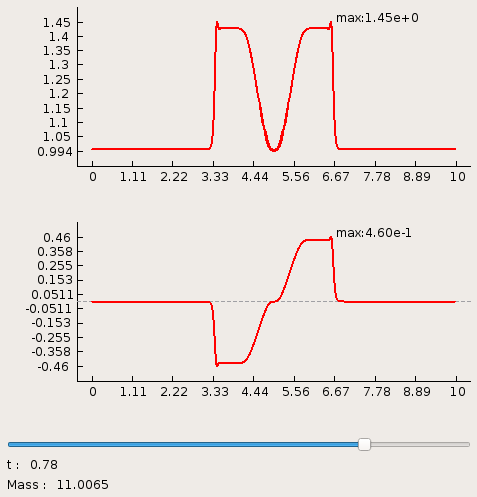
\includegraphics[width=1\linewidth]{p1/p1_t=0,78.png}
	\end{minipage}
	\begin{minipage}[h] {0.49\linewidth}
		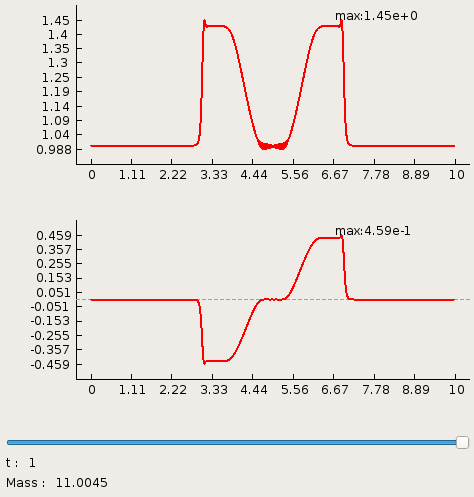
\includegraphics[width=1\linewidth]{p1/p1_t=1.png}
	\end{minipage}
	\caption{Графики плотности (верхний) и скорости (нижний)}
\end{figure}
Заметим, что закон сохранения масс выполнен, т.к. изменяется в пределах вычислительной погрешности.

Для задачи (2) получаем:
\begin{figure}[H]
	\begin{minipage}[h] {0.49\linewidth}
		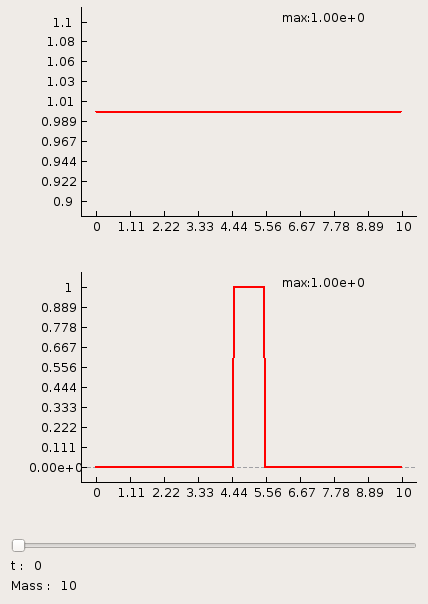
\includegraphics[width=1\linewidth]{p2/p2_t=0.png}
	\end{minipage}
	\begin{minipage}[h] {0.49\linewidth}
		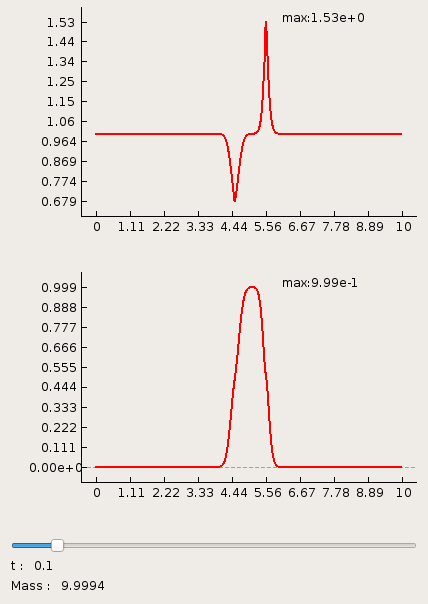
\includegraphics[width=1\linewidth]{p2/p2_t=0,1.png}
	\end{minipage}
\end{figure}
\begin{figure}[H]
	\begin{minipage}[h] {0.49\linewidth}
		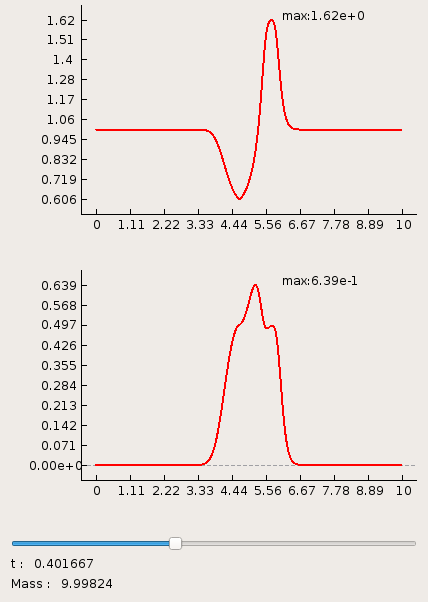
\includegraphics[width=1\linewidth]{p2/p2_t=0,4.png}
	\end{minipage}
		\begin{minipage}[h] {0.49\linewidth}
		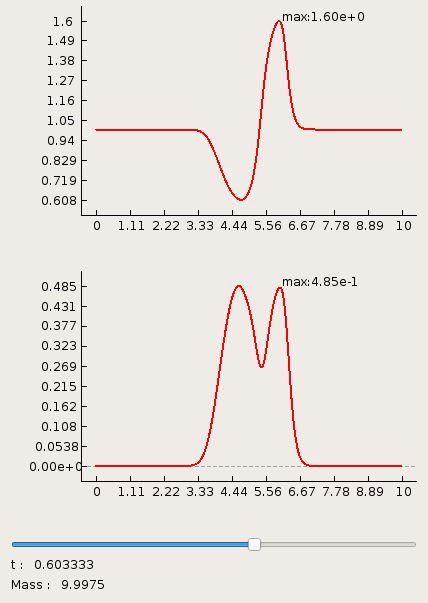
\includegraphics[width=1\linewidth]{p2/p2_t=0,6.png}
	\end{minipage}

	\begin{minipage}[h] {0.49\linewidth}
		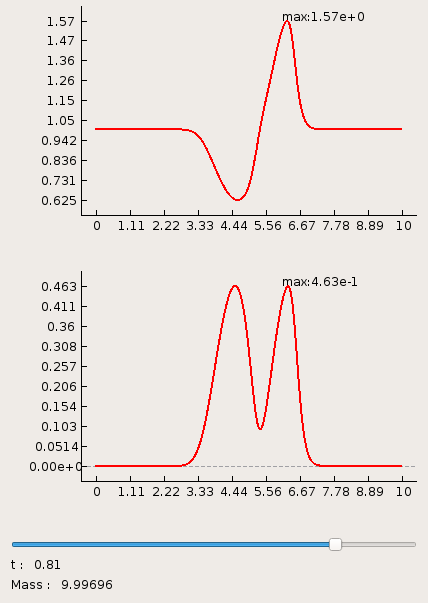
\includegraphics[width=1\linewidth]{p2/p2_t=0,8.png}
	\end{minipage}
	\begin{minipage}[h] {0.49\linewidth}
		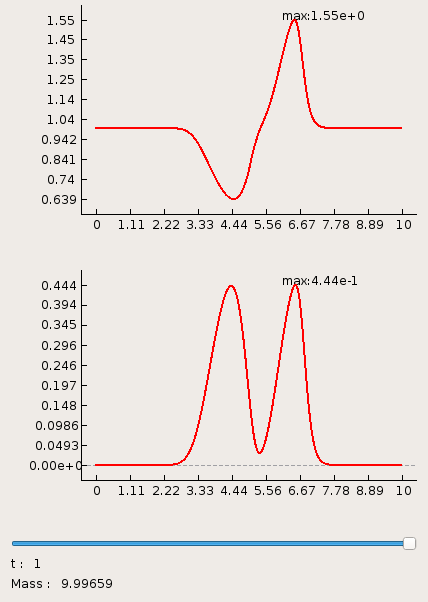
\includegraphics[width=1\linewidth]{p2/p2_t=1.png}
	\end{minipage}
	\caption{Графики плотности (верхний) и скорости (нижний)}
\end{figure}
Закон сохранения массы так же выполнен.

\section{Зависимость точности полученного решения от коэффициента вязкости газа}

\begin{tabular}{|l|c|c|c|}
\hline
норма $\backslash \ \mu$ 					& 0.001      & 0.01       & 0.1 \\
\hline
$\|G_m^n - g (\tau n, hm)|_{C_h}$ 			& 2,584176e-04 & 3,700739e-04 & 2,817834e-03 \\
\hline
$\|G_m^n - g (\tau n, hm)|_{L_{2,h}}$ 		& 3,207805e-04 & 4,151149e-04 & 2,019011e-03 \\
\hline
$\|G_m^n - g (\tau n, hm)|_2^1$ 			& 5,062162e-04 & 7,514924e-04 & 5,873506e-03 \\
\hline
$\|V_m^n - u (\tau n, hm)|_{C_h}$ 			& 4,216830e-04 & 4,278619e-04 & 2,062970e-03 \\
\hline
$\|V_m^n - u (\tau n, hm)|_{L_{2,h}}$ 		& 6,341970e-04 & 6,255225e-04 & 1,524787e-03 \\
\hline
$\|V_m^n - u (\tau n, hm)|_2^1$ 			& 7,866074e-04 & 8,754409e-04 & 5,837614e-03 \\
\hline
\end{tabular}\\

\section{Стабилизация газа на негладких начальных условиях}
Интересно построить решение разностной схемы на области, неограниченной по времени. Вместо этого критерием окончания итеративного процесса, может являться достаточно малая разность между максимальным и минимальным значением плотности газа на $[0, X]$. Приведем графические результаты работы алгоритма на задаче (4.1) с критерием для плотности $\varepsilon = 10^-2$.
\begin{figure}[H]
	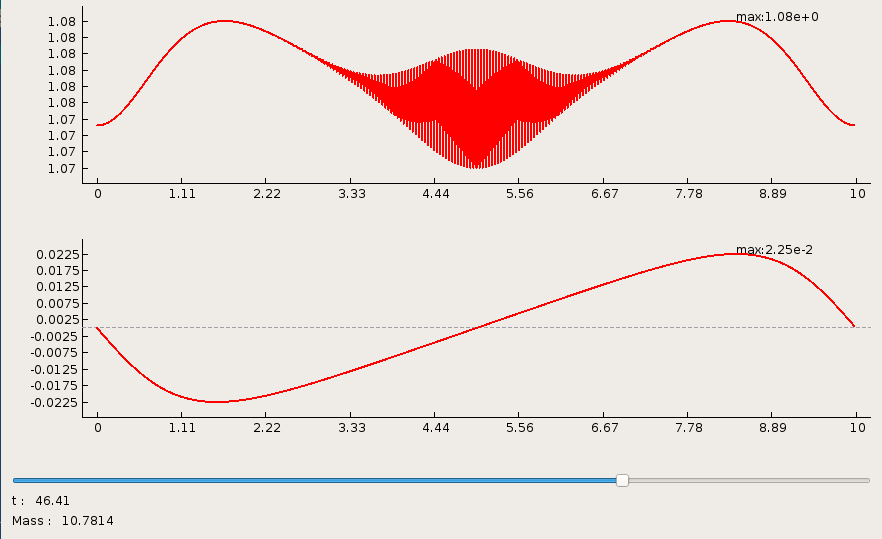
\includegraphics[width=1\linewidth]{p3/p3_rho_t=46,41.png}
\end{figure}
Отметим, что осцилляции в области начального скачка плотности являются малыми (порядка $0,01$) по сравнению со значениями плотности ($\rho \approx 1$), и являются следствием естественной погрешности алгоритма.


\end{document}
